\begin{figure}[tbp!]
    \centering
    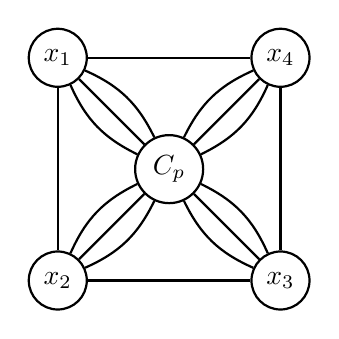
\begin{tikzpicture}[node distance={20mm}, thick, main/.style = {draw, circle}] 
        \node[main] (C) {$C_p$};
        \node[main] (1) [above left of=C] {$x_1$}; 
        \node[main] (2) [below left  of=C] {$x_2$};
        \node[main] (3) [below right of=C] {$x_3$}; 
        \node[main] (4) [above right of=C] {$x_4$};
        \draw (1) -- (2);
        \draw (2) -- (3);
        \draw (4) -- (3);
        \draw (1) -- (4);
        
        \draw (1) -- (C);
        \path[-] (1) edge [bend left=20] node {} (C);
        \path[-] (1) edge [bend right=20] node {} (C);

        \draw (2) -- (C);
        \path[-] (2) edge [bend left=20] node {} (C);
        \path[-] (2) edge [bend right=20] node {} (C);
        
        \draw (3) -- (C);
        \path[-] (3) edge [bend left=20] node {} (C);
        \path[-] (3) edge [bend right=20] node {} (C);

        \draw (4) -- (C);
        \path[-] (4) edge [bend left=20] node {} (C);
        \path[-] (4) edge [bend right=20] node {} (C);
    \end{tikzpicture}
    \caption{The graph $\G_0$ depicted here is a subgraph of the complete graph $\G$ which encodes a constant number of independence constraints as $p$ grows.}
    \label{fig-graph-exp-1}
\end{figure}